\section{Artificial Intelligence: Multi-class Classification}

In the previous project review, we introduced a Convolutional Neural Network (CNN) classification algorithm that demonstrated promising results for single-class classification. However, our project's goal extended beyond single-class classification; we aimed to implement a multi-class classification system.\\

\noindent In our case of road damage detection, the goal is to accurately identify various types of road deteriorations within a continuous sequence of accelerometric records. Each segment in the sequence represents a unique class corresponding to different types of road damage, such as potholes, cracks, bumps, or other forms of degradation.

Assigning multiple classes to one instance requires a sophisticated approach in the model architecture. It necessitates a deep learning model capable of understanding and classifying distinct segments within a continuous stream of data, allowing for the simultaneous identification of multiple classes.

\subsection{Sliding Window: CNN - Sliding Window Approach}

We aimed to implement this system, with the idea of utilizing a sliding window approach. Although discussions with our project jury emphasized that segmentation might be a more effective method, we were faced with considerable challenges in implementing a segmentation algorithm. Given that we had already initiated the development of a sliding window algorithm, we were determined to see it through. In this section, we will elucidate the concept of the sliding window algorithm, its implementation, and the results obtained.

\subsubsection{Sliding Window Algorithm Concept}
The sliding window algorithm operates by applying a classification model to a long sequence. Unlike traditional classification methods that analyze data as a whole, the sliding window approach segments the data by moving a window of predefined size and step length across the sequence. As the window slides, the model performs classification within each window, effectively breaking the data into smaller sections.

\subsubsection{Algorithm Implementation}
Our journey with the sliding window approach began by concatenating five random basic data sequences and manually labeling the different sections within the concatenated data sequence.
\begin{figure}[H]
    \centering
    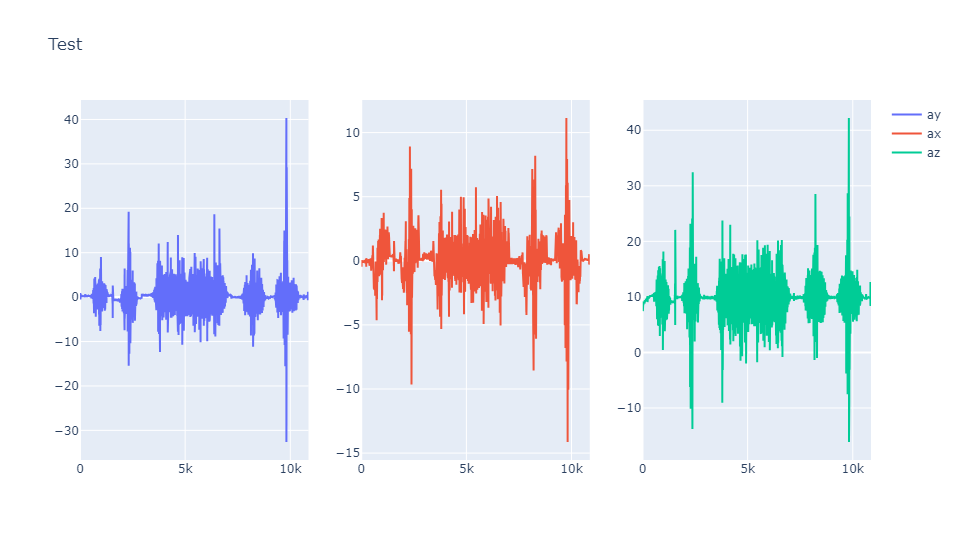
\includegraphics[width=0.5\linewidth]{concat.png}
    \caption{Concatenated Data Sequence}
    \label{fig:enter-label}
\end{figure}

We assigned labels such as 1, 2, 1, 4, and 4 to these segments based on their characteristics.
\begin{figure}[H]
    \centering
    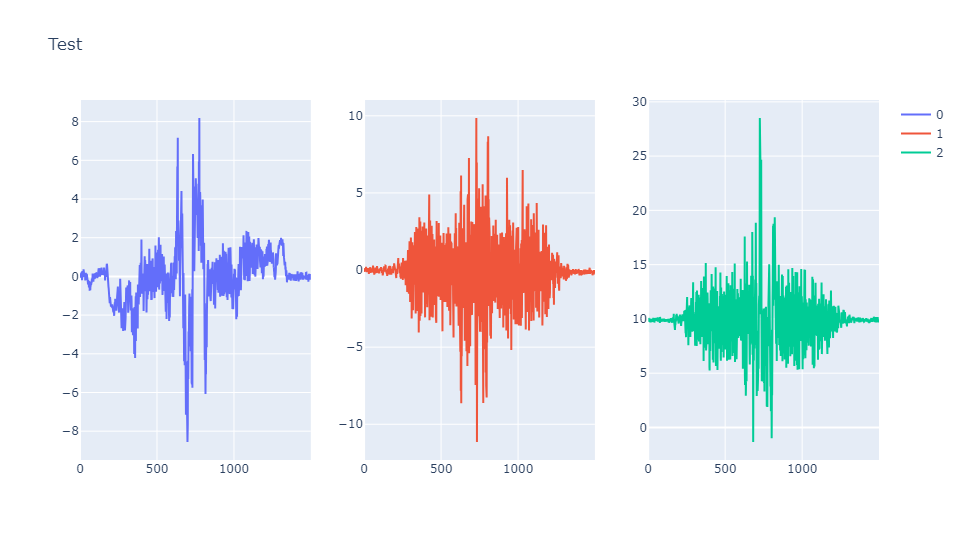
\includegraphics[width=0.5\linewidth]{petite.png}
    \caption{Cut of the concatenated data from data 7500 to 9000, here the predicted class is 4}
    \label{fig:enter-label}
\end{figure}

To implement the sliding window algorithm, we utilized the CNN model, fine-tuning it to handle this segmentation task. Significant effort was invested in finding the optimal window size and step length to ensure accurate classification.

We also introduced a threshold in the predicted probabilities to determine whether a label should be assigned or not. This addition allowed us to avoid forcing the algorithm to assign a label in situations where one might not be present.

\subsubsection{Results and Visualization}
To evaluate the algorithm's performance, we generated both graphical and label-based results. The graphical representation showed the progression of the sliding window across the data sequence, while the labels assigned by the model were displayed as colored squares at specific locations along the sequence.
\begin{figure}[H]
    \centering
    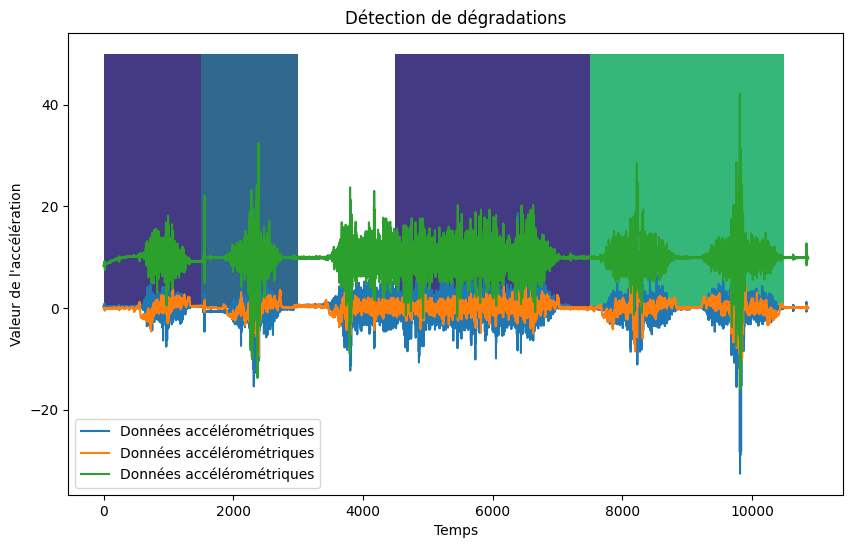
\includegraphics[width=0.5\linewidth]{sliding.png}
    \caption{Visualisation of the Sliding Window Result}
    \label{fig:enter-label}
\end{figure}


While the detected labels may not precisely align with the actual regions of road damage due to the size of the windows, the results were encouraging. The algorithm found the same sequence as the one found manually. It's worth noting that issues can arise with very long sequences, where a label may span multiple windows and, as a result, go undetected.

Although our initial results are promising, they are not without limitations, especially in the context of long sequences. As a result, we acknowledge that while the sliding window approach has merits, it may not be sufficient for our project's comprehensive objectives. Therefore, we remain committed to exploring other methodologies, particularly segmentation, to enhance the accuracy and efficiency of road damage classification in our project.


\subsection{Segmentation: CNN}

\subsubsection{Algorithm Concept: Segmentation in Deep Learning}

Segmentation in the context of deep learning involves the division of an input sequence into distinct segments, with each segment belonging to a specific class or category. Unlike traditional classification methods where an entire sequence is labeled as a single class, segmentation assigns multiple classes to different sections within the sequence.

The CNN employed in this context is designed to recognize patterns and features within segments of the data sequence, enabling the model to distinguish between different types of road damage. This multi-class classification capability is crucial in accurately identifying and labeling various segments in the sequence, contributing to more comprehensive road damage detection.

By segmenting the input sequence and assigning multiple classes to each segment, the deep learning model gains the ability to capture and classify diverse features present in the data, resulting in a more nuanced and detailed understanding of different types of road damage within the given sequence.

\subsubsection{Algorithm Implementation}

The model employed a sequence of convolutional layers, batch normalization, and ReLU activation functions for feature extraction and dimensionality reduction. The model's final output layer was structured for multi-class classification, enabling the identification of various types of road deteriorations.

\begin{figure}[H]
  \centering
  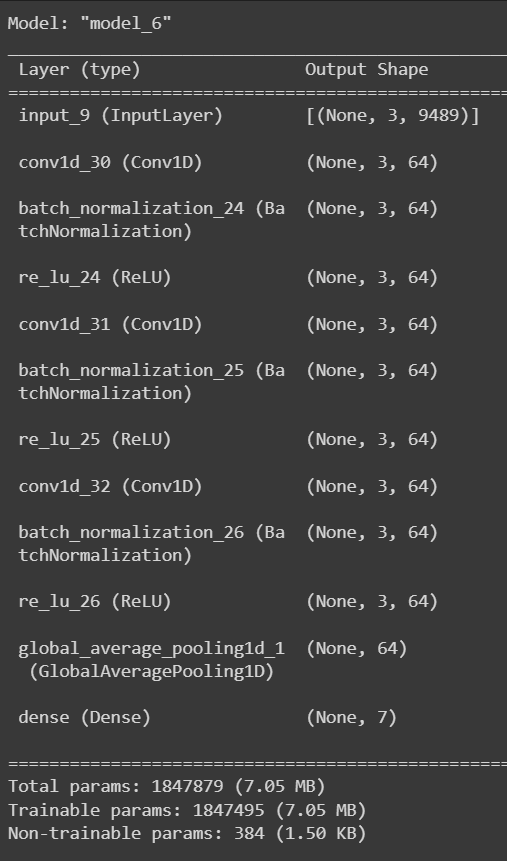
\includegraphics[width=0.4\textwidth]{img/SegCNNmodel.png}
  \caption{Structure of the CNN Segmentation Model}
  \label{SegCNNEval}
\end{figure}

The training phase involved compiling, fitting, and optimizing the model using encoded multi-class labels and categorical cross-entropy as the loss function. Training and validation data were properly formatted to comply with the input structure expected by the model.

The model training process encompassed several epochs, with continuous validation to ensure model accuracy and prevent overfitting. The trained model was then evaluated using a separate test dataset, providing insight into its accuracy and loss metrics.

\subsubsection{Results}

\noindent \textbf{Overfitting Analysis}\\

\noindent The model training process for the CNN-based segmentation encountered signs of overfitting. At the initial epochs, the training phase reflected a substantial improvement in accuracy, while the validation accuracy remained stagnant or even declined. This discrepancy in the accuracies between the training and validation data suggested the model had memorized the training data excessively and was not generalizing well to new, unseen data.

\begin{figure}[H]
  \centering
  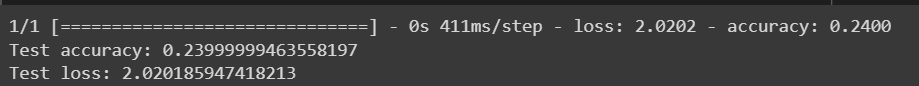
\includegraphics[width=0.75\textwidth]{img/SegCNNEval.png}
  \caption{Evaluation of the CNN Segmentation Model}
  \label{SegCNNEval}
\end{figure}

\noindent During the training period of 500 epochs, the model displayed a notable rise in accuracy, reaching a perfect accuracy score on the training data. However, this sharp improvement did not align with the validation set, where accuracy remained relatively unchanged.

\begin{figure}[H]
  \centering
  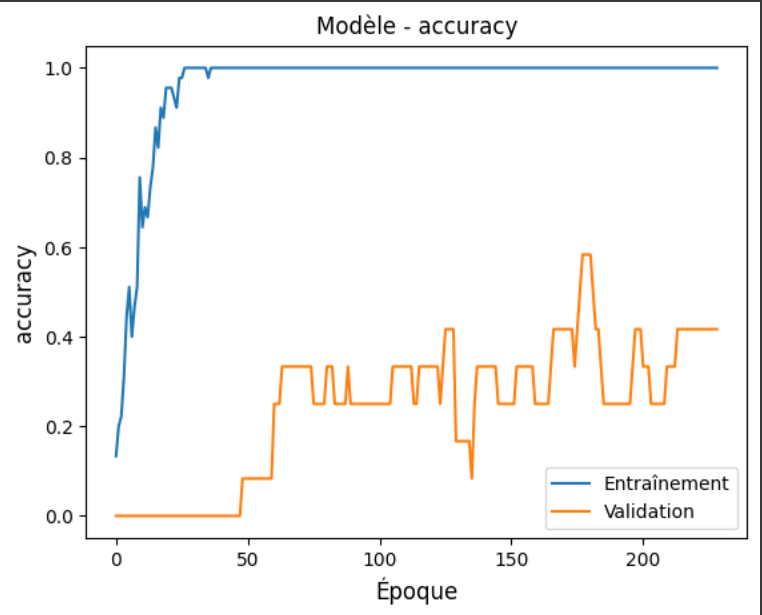
\includegraphics[width=0.5\textwidth]{img/SegCNNGraph.png}
  \caption{Graphical Visualization of CNN Segmentation Model Learning and Evaluation}
  \label{SegCNNGraph}
\end{figure}

\noindent The model's evaluation stage further confirmed this trend, where the accuracy on the test data remained considerably lower compared to the accuracy seen on the training data. Therefore, it can be concluded that the model experienced overfitting, implying the need for regularization techniques or model adjustments to prevent the learning process from focusing too heavily on the training data's specific details.